




 Consider the following triangle:
 \begin{center}
 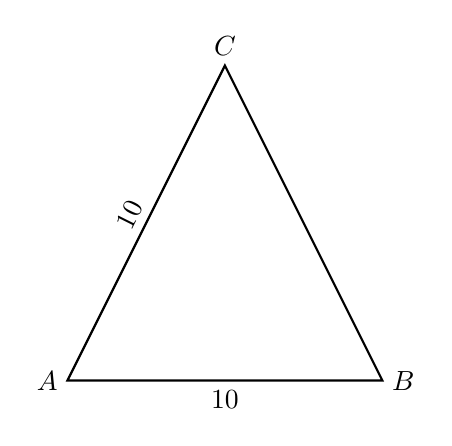
\begin{tikzpicture}
 
 \draw (0,0) --(2,4)--(4,0)--cycle  [thick,-,>=latex];
  \draw node[above] at (2,4) {$C$};
  \draw node[left] at (0,0) {$A$};
  \draw node[right] at (4,0) {$B$};
 
 
   \draw (0,0)--(2,4) node[above,midway, sloped]{$10$};
   \draw (0,0)--(4,0) node[below,midway, sloped]{$10$};


\end{tikzpicture}
\end{center}
If $m\angle A=60^\circ$, then what is the perimeter of this triangle?


\ifsat
	\begin{enumerate}[label=\Alph*)]
		\item  $30$%
		\item $50$
		\item $75$
		\item  Cannot be determined
	\end{enumerate}
\else
\fi

\ifacteven
	\begin{enumerate}[label=\textbf{\Alph*.},itemsep=\fill,align=left]
		\setcounter{enumii}{5}
		\item  $30$%
		\item $50$
		\item $60$
		\addtocounter{enumii}{1}
		\item $75$
		\item  Cannot be determined
	\end{enumerate}
\else
\fi

\ifactodd
	\begin{enumerate}[label=\textbf{\Alph*.},itemsep=\fill,align=left]
		\item  $30$%
		\item $50$
		\item $60$
		\item $75$
		\item  Cannot be determined
	\end{enumerate}
\else
\fi

\ifgridin
  $30$%
		
\else
\fi

